\begin{figure}\centering
% Define some block styles
\tikzstyle{title} = [%
	rectangle,%
%	minimum height=2em,%
	text centered%
]
\tikzstyle{function} = [%
	rectangle,%
	draw,%
	fill=white,%
%	minimum height=2em,%
	rounded corners=5pt,%
]

\begin{tikzpicture}[node distance=3cm, shorten >= 1pt, >=stealth', auto, anchor=west]
	
	\def\title_offset{-1.33};
	\def\image_offset{-2.66};
	
	\node at (0, 0) (closed_loop_optimisation) [title] {Closed-Loop Optimisation};

	\node at (0, \title_offset+\image_offset) (opendss_logo) [rectangle] {
\includegraphics[height=7.5mm]{_chapter1/fig/OpenDSS}};
	\node (simulation_text) [rectangle, right of=opendss_logo, xshift=-1.5cm] {Simulation};
	\node (simulation) [function, fit={(opendss_logo) (simulation_text)}] {};
	\node at (0, \title_offset+\image_offset) (opendss_logo) [rectangle] {
\includegraphics[height=7.5mm]{_chapter1/fig/OpenDSS}};
	\node (simulation_text) [rectangle, right of=opendss_logo, xshift=-1.5cm] {Simulation};
	
	\node at (0, \title_offset) (matlab_cost) [rectangle] {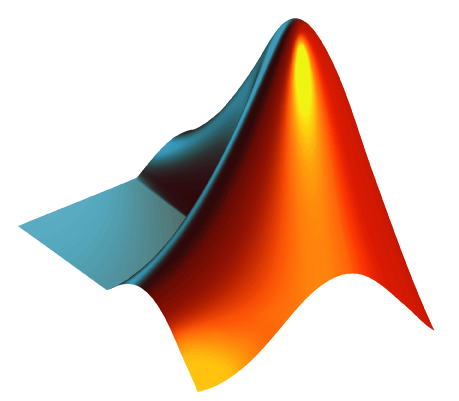
\includegraphics[height=7.5mm]{_chapter1/fig/MATLAB}};
	\node (cost_function_text) [rectangle, right of=matlab_cost, xshift=-1.15cm] {Cost Function};
	\node (cost_function) [function, fit={(matlab_cost) (cost_function_text)}] {};
	\node at (0, \title_offset) (matlab_cost) [rectangle] {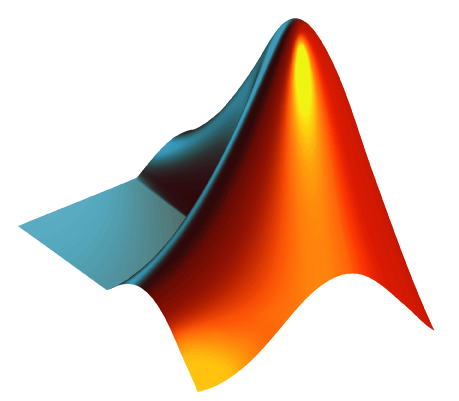
\includegraphics[height=7.5mm]{_chapter1/fig/MATLAB}};
	\node (cost_function_text) [rectangle, right of=matlab_cost, xshift=-1.15cm] {Cost Function};
	
	\node at (7, \title_offset) (matlab_optimiser) [rectangle] {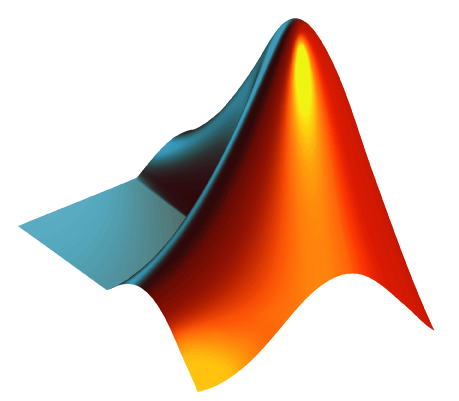
\includegraphics[height=7.5mm]{_chapter1/fig/MATLAB}};
	\node (optimiser_text) [rectangle, right of=matlab_optimiser, xshift=-1.5cm] {Optimiser};
	\node (optimiser) [function, anchor=center, fit={(matlab_optimiser) (optimiser_text)}] {};
	\node at (7, \title_offset) (matlab_optimiser) [rectangle] {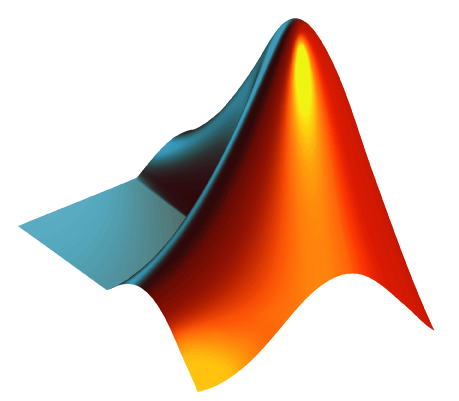
\includegraphics[height=7.5mm]{_chapter1/fig/MATLAB}};
	\node (optimiser_text) [rectangle, right of=matlab_optimiser, xshift=-1.5cm] {Optimiser};
	
	\node at (8, \title_offset+\image_offset) (addition) [state, fill=white] {$+$};
	
	\node at (12.5, \title_offset-2) (battery) [rectangle] {
\includegraphics[height=15mm]{_chapter1/fig/battery}};
	\node (model_text) [rectangle, below of=battery, yshift=1.9cm] {Model};
	\node (model) [function, fit={(battery) (model_text)}] {};
	\node at (12.5, \title_offset-2) (battery) [rectangle] {
\includegraphics[height=15mm]{_chapter1/fig/battery}};
	\node (model_text) [rectangle, below of=battery, yshift=1.9cm] {Model};
	
	\node (output) [function, below of=addition, fill=yellow!20, yshift=1cm, inner sep=1em] {Output};
	
	\begin{scope}[on background layer]
		\node [draw=black, fill=green!20, fit={%
			(closed_loop_optimisation)%
			(simulation)%
			(cost_function)%
			(optimiser)}] {};
	\end{scope}

	\draw [->, bend left] (simulation) to node {key parameters} (cost_function);
	\draw [->] (cost_function) to node [above] {$\zeta(\boldsymbol{\alpha})$} (optimiser);
	\draw [->, bend left] (optimiser) to node [left] {$\delta \textbf{s}_{ESMU}(t)$} (addition);
	\draw [->] (addition) to node [above] {$\textbf{s}_{ESMU}(t) + \delta \textbf{s}_{ESMU}(t)$} (simulation);
	\draw [->] (model.west|-addition) to node [above, pos=0.3] {$\textbf{s}_{ESMU}(t)$} (addition);
	\draw [->, dashed, bend right, color=red] (model) to node [midway, above, yshift=1mm] {constraints} (optimiser.east|-optimiser.center);
	\draw [->] (addition) -- (output);
\end{tikzpicture}
\caption{ESMU schedule adjustment flow diagram}
\label{ch1:fig:closed-loop-optimisation}
\end{figure}